\documentclass[11pt]{article}

\usepackage[margin=2cm]{geometry}
\usepackage{graphicx}
\usepackage{booktabs}
\usepackage{hyperref}
\usepackage{enumitem}
\usepackage{microtype}

\setlist{nosep}
\setlength{\parindent}{0pt}
\setlength{\parskip}{0.5em}

\title{MAC0623 - 3D Interaction in Mixed Realities \\ Assignment 1: Desktop Docking Testbed}
\author{Leonardo Heidi Almeida Murakami - NUSP: 11260186}
\date{}

\begin{document}

\maketitle

\noindent
\textbf{Public URL:}
\url{https://leonardomurakami.github.io/mac0623-a1/}

\textbf{Repository:}
\url{https://github.com/leonardomurakami/mac0623-a1}

\textbf{Browsers tested:} Firefox and Chrome on Windows

\begin{abstract}
I compared two mouse mappings for a 6-DoF docking task, where the user must
match a cube's position and orientation to a target.

The baseline switches between translation and rotation modes, while my
mapping uses a 3D gizmo with separate handles for each axis. I expected the
gizmo to improve accuracy at a small cost in speed.

With 5 participants and 31 recorded trials, the gizmo produced substantially
lower position and orientation errors. Completion time was similar overall,
although the effect on speed varied considerably between participants.
\end{abstract}

\section{Method}

The experiment was implemented in Three.js and run in Firefox and Chrome on
Windows. The target tolerance was 0.05 scene units for position and
$10^\circ$ for orientation.

The two mappings were:

\begin{itemize}
    \item \textbf{Baseline:} Spacebar or Tab switches between translation
    and rotation. Mouse movement controls two axes and the mouse wheel
    controls the third.

    \item \textbf{Gizmo:} Spacebar or Tab switches between translation and
    rotation handles. The user selects an axis handle and drags it, changing
    only that axis.
\end{itemize}

I tested 5 participants recruited from friends. Three were Computer Science
students, one was a medical student, and one was from outside the CS group.
P01 and P02 used the gizmo first, while P03, P04, and P05 used the baseline
first.

Each participant received one untimed practice trial per mapping followed by
three timed trials. One additional baseline trial from P03 was recorded, so
the dataset contains 31 trials in total. No coaching was given during timed
trials.

For each trial I recorded completion time, final position error, final
orientation error, mode switches, and path length.

\section{Results}

\begin{figure}[ht]
    \centering
    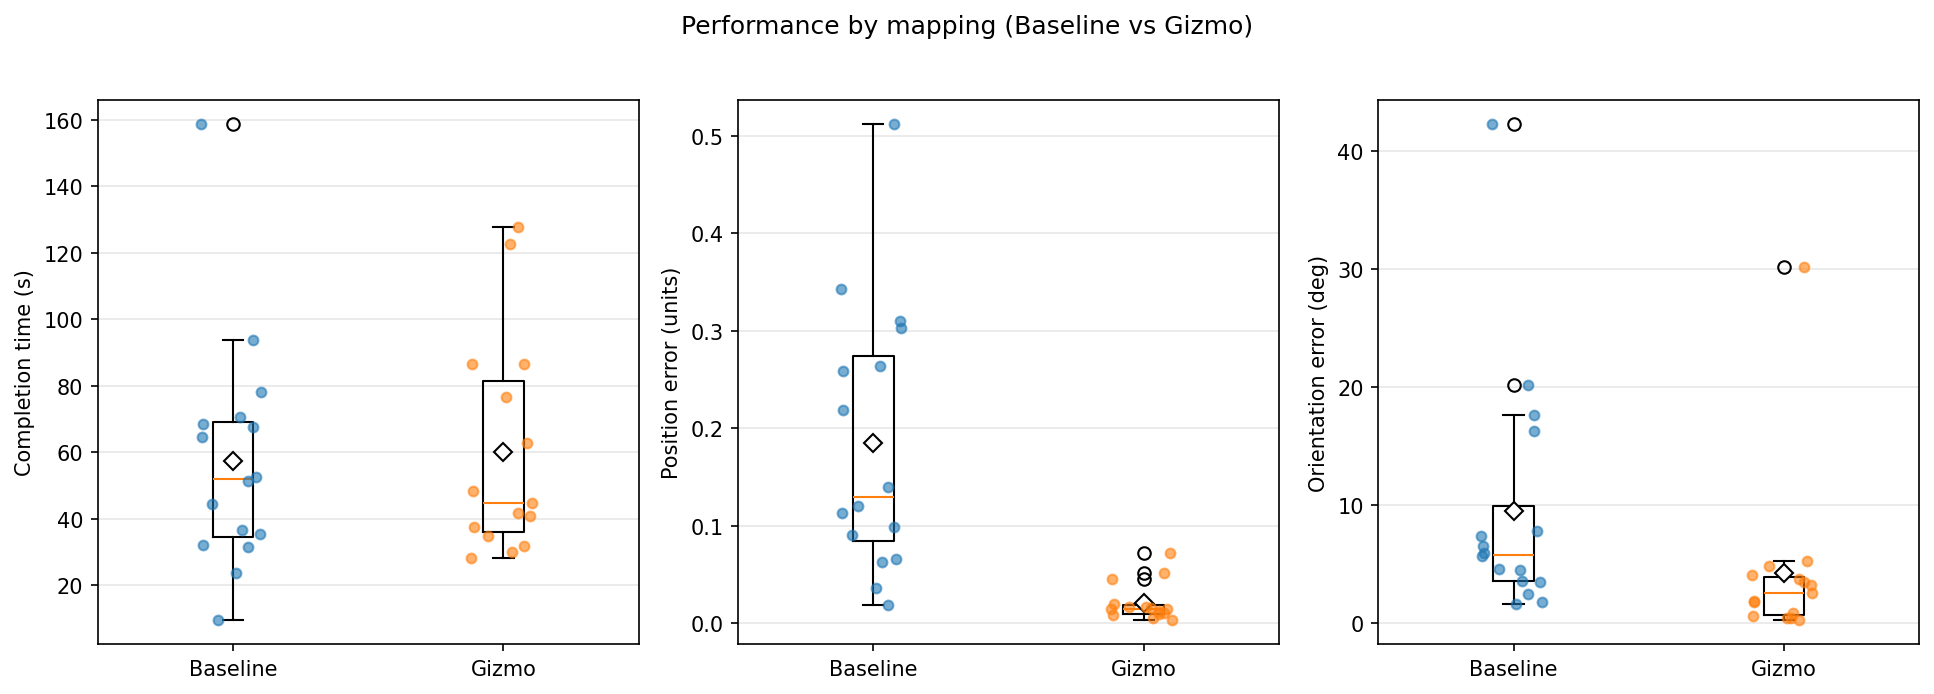
\includegraphics[width=0.9\textwidth]{plots/combined.png}
    \caption{Performance by mapping.}
    \label{fig:results}
\end{figure}

\begin{table}[ht]
\centering
\begin{tabular}{lrrr}
\toprule
\textbf{Metric} & \textbf{Baseline} & \textbf{Gizmo} & \textbf{$n$} \\
\midrule
Completion time &
$57.45 \pm 34.95$ s &
$60.04 \pm 32.87$ s &
16 / 15 \\

Position error &
$0.185 \pm 0.137$ &
$0.021 \pm 0.019$ &
16 / 15 \\

Orientation error &
$9.49^\circ \pm 10.45^\circ$ &
$4.23^\circ \pm 7.37^\circ$ &
16 / 15 \\

Mode switches &
$5.75 \pm 4.65$ &
$4.20 \pm 2.60$ &
16 / 15 \\
\bottomrule
\end{tabular}
\caption{Mean $\pm$ standard deviation. The final column shows
Baseline / Gizmo trial counts.}
\label{tab:results}
\end{table}

Because participants completed both mappings, I also compared each
participant's mean performance. On average, the gizmo was 2.16 s slower,
reduced position error by 0.165 units, and reduced orientation error by
$5.72^\circ$.

Position accuracy was the clearest result. Every participant had lower
position error with the gizmo, and the overall mean fell from 0.185 to
0.021, an improvement of about 8.8 times.

Orientation accuracy also improved for every participant except P02.
Overall mean orientation error fell from $9.49^\circ$ to $4.23^\circ$.

Speed was less consistent. P01, P02, and P03 were slower with the gizmo,
while P04 and P05 were faster. The largest differences were P03, who was
about 58 s slower, and P04, who was about 67 s faster.

\section{Discussion}

The gizmo clearly performed better on \textbf{accuracy}, while neither
mapping clearly won on \textbf{speed}. This partially supports my original
prediction: the expected accuracy improvement appeared strongly in the
data, but the speed cost was small overall and depended heavily on the
participant.

The position result fits the motivation for the design. The baseline has a
\textbf{DoF mismatch}: a 2D mouse controls a 6-DoF task by decomposing it
into translation and rotation modes. The gizmo decomposes it further, with
one axis controlled per drag. This prevents a correction on one axis from
changing another, which likely explains the much smaller position errors.

Orientation showed a similar but weaker effect. Four of the five
participants improved with the gizmo. P02 was the exception, with mean
orientation error increasing from $8.48^\circ$ to $11.31^\circ$. This may
indicate a cost in learning or selecting the rotation handles: constraining
the movement helps only after the user understands which ring controls each
axis.

The speed results were more surprising. P03 was much slower with the gizmo,
suggesting that selecting individual handles added substantial overhead.
P04 showed the opposite behavior, dropping from a mean of 101.7 s with the
baseline to 34.9 s with the gizmo. For this participant, avoiding repeated
corrections appears to have saved more time than handle selection cost.

There are several limitations. The sample is still small and was recruited
from my own friends rather than randomly. Three participants were CS
students, so familiarity with interfaces similar to 3D editing tools may
also affect the results. The mapping order was counterbalanced as evenly as
possible with five participants, but practice effects may still remain.
Finally, one additional baseline trial was recorded for P03, producing
slightly unequal trial counts between mappings.

All of the participants said that the Gizmo was more intuitive to learn and
control the cube while the Baseline was extremely confusing and frustrating because
it felt unnatural.

\end{document}